\section{Experiments}
\label{sec:experiments}

\subsection{Protocol}
\label{sec:protocol}
\paragraph{Datasets.}
\vxreal~\cite{xiang2024v2xreal} is real traffic with two vehicles and two infrastructure units per scenario; we use the official 48 / 6 / 14 train / val / test scenarios (2,172 test frames, \SI{70}{m} communication range, one vehicle class). \opvv~\cite{xu2022opv2v} is CARLA-simulated V2V traffic; its \texttt{validate} split is a copy of \texttt{test}, so we hold out a scenario-disjoint 15\% of the training scenarios for every selection and report on the official 2,170 test frames. Nothing below is selected on test.

\paragraph{Detector and fusion.}
A PointPillars~\cite{lang2019pointpillars} detector per agent, trained from scratch on each dataset at the full evaluated range, is shared by every method; the fusion stage, NMS over the union of corrected boxes, is also shared. All differences in the tables come from the alignment step alone.

\paragraph{Noise.}
Each CAV pose is perturbed with zero-mean Gaussian noise of standard deviation $\sigma$ metres in $x$ and $y$ and $\sigma$ degrees in yaw, $\sigma\in\{0,0.2,0.4,0.6,0.8,1,1.5,2\}$. Draws are keyed on (seed, $\sigma$, frame, agent), so every method inside one run sees the same perturbed pose and differences between methods are paired; we report five seeds on test and three on validation, and the paired per-seed difference is the statistic. The clean cell is deterministic and run once. Delay is modelled as the CAV transmitting what it saw $d$ frames earlier with its pose at that time, $d\in\{1,2,4\}$ at \SI{10}{Hz}.

\paragraph{Metrics.}
Globally confidence-sorted AP at IoU 0.3, 0.5 and 0.7 over the full test set, per $\sigma$ and as the mean over the sweep. We additionally split frames by the number of ground-truth objects the ego and the CAV share, into 0, 1--2 and 3+, because the two alignment families fail in different buckets. Pose error is reported only as a diagnostic.

\paragraph{Baselines.}
\freealign~\cite{lei2024freealign} is reimplemented onto our detections, sweep and evaluator; its code is bound to a different detector, postprocessor and AP implementation, and running it end to end would not isolate the alignment algorithm. Its six parameters (edge feature, edge threshold, anchor limit, score offset and power, robust estimator) are selected on validation. We found the selection criterion matters: the natural one for a pose estimator, mean pose error, picks a \SI{0.3}{m} edge threshold at which \freealign answers 29\% of \vxreal pairs; selecting the threshold by \freealign's \emph{own validation AP} picks \SI{1.0}{m} (60\% coverage) and is worth +0.061 \ap{0.7} on test. Every \freealign number in this paper is the AP-selected one; the pose-error-selected one is in the supplement. On \opvv we also run seven intermediate-fusion methods under the same sweep: AttFuse~\cite{xu2022opv2v}, V2X-ViT~\cite{xu2022v2xvit}, CoBEVT~\cite{xu2022cobevt}, CoAlign's fusion~\cite{lu2023coalign}, Where2comm~\cite{hu2022where2comm}, F-Cooper~\cite{chen2019fcooper} and V2VAM~\cite{li2023v2vam}, from OpenCOOD checkpoints trained at the same range. The \emph{oracle} corrects every CAV with its true pose and is the ceiling of any aligner; \emph{uncorrected} is late fusion as deployed.

\subsection{Main result on \vxreal}
\label{sec:main}

\begin{table*}[t]
  \centering\small
  \caption{\textbf{\vxreal test, \ap{0.7} against localization noise} (2,172 frames, 5 paired noise seeds; paired standard errors of the sweep-mean differences are $\le 0.0005$). \freealign at its AP-selected threshold. Rows above the rule are the stages of \paper in order; the last is the full method, the one rule selected on validation of both datasets (Sec.~\ref{sec:ablation}). The agreement row is from the RANSAC run; the least-squares row from the earlier run with the same seeds.}
  \label{tab:main}
  \begin{tabular}{l*{8}{c}c}
    \toprule
    $\sigma$ (m / deg) & 0 & 0.2 & 0.4 & 0.6 & 0.8 & 1.0 & 1.5 & 2.0 & mean \\
    \midrule
    uncorrected late fusion & .4223 & .3185 & .2155 & .1771 & .1621 & .1580 & .1584 & .1632 & .2219 \\
    oracle (true pose) & \multicolumn{8}{c}{.4223 at every $\sigma$} & .4223 \\
    \freealign (AP-selected, \SI{1.0}{m}) & .3702 & .3577 & .3420 & .3362 & .3331 & .3321 & .3303 & .3301 & .3415 \\
    \midrule
    propose (Wald $\alpha{=}0.2$) & .3932 & .3404 & .3100 & .3032 & .2993 & .2940 & .2797 & .2661 & .3107 \\
    + verify (ICP, least squares) & .4024 & .3519 & .3269 & .3237 & .3236 & .3239 & .3220 & .3188 & .3366 \\
    + verify (two-point RANSAC, \SI{6}{m} schedule) & \best{.4057} & .3554 & .3288 & .3265 & .3259 & .3265 & .3274 & .3267 & .3404 \\
    + agreement \SI{1.0}{m} & .3902 & .3695 & .3478 & .3413 & .3321 & .3278 & .3149 & .3053 & .3411 \\
    + consensus floor 4 & .3893 & .3721 & .3553 & .3501 & .3456 & .3428 & .3385 & .3349 & .3536 \\
    \textbf{+ weighted refit (\paper)} & .3921 & \best{.3750} & \best{.3576} & \best{.3525} & \best{.3466} & \best{.3445} & \best{.3400} & \best{.3360} & \best{.3555} \\
    \bottomrule
  \end{tabular}
\end{table*}

\begin{table}[t]
  \centering\small
  \caption{\textbf{\vxreal test, sweep means at three IoU thresholds.} Paired standard errors over five seeds.}
  \label{tab:thresholds}
  \resizebox{\linewidth}{!}{\begin{tabular}{lccc}
    \toprule
    & \ap{0.7} & \ap{0.5} & \ap{0.3} \\
    \midrule
    uncorrected & .2219 & .3665 & .4676 \\
    \freealign (AP-selected) & .3415 & .4933 & .5390 \\
    propose & .3107 & .4854 & .5502 \\
    propose + verify (LS) & .3366 & .5038 & .5583 \\
    propose + verify (RANSAC) & .3404 & .5100 & .5642 \\
    propose + verify + agree & .3411 & .5029 & .5537 \\
    + consensus floor & .3536 & \best{.5196} & \best{.5671} \\
    \textbf{\paper} (+ weighted refit) & \best{.3555} & .5185 & .5663 \\
    \quad paired difference to \freealign & $+.0141\pm.0001$ & $+.0255\pm.0002$ & $+.0282\pm.0003$ \\
    \bottomrule
  \end{tabular}}
\end{table}

Table~\ref{tab:main} reads top to bottom as the method was built. The learned proposal alone wins the clean case by 0.023 over \freealign and loses the noisy sweep by 0.031: the soft fit is blurred where \freealign's hard fit is sharp. The exact verification recovers 0.026 of that (paired, $\pm0.0003$) and reverses the order at IoU 0.5 and 0.3. The agreement rule adds 0.004 by declining the pairs where the two estimates disagree. The consensus floor adds 0.012 on the sweep mean, and weighting the exact refit by the soft solve's confidence precisions another 0.002, to a paired lead of $+0.0141\pm0.0001$ over \freealign, ahead at every $\sigma$ including the clean case (.392 against .370) and by 0.006 at \SI{2}{m}; at IoU 0.5 and 0.3 the lead is 0.026 and 0.028 and holds at every $\sigma$ (Table~\ref{tab:thresholds}). The order of the arms on test is the order on validation, where the same rule was +0.0097 and the floor was selected among $\{0,4,6\}$.

\paragraph{Where the two families fail.}
Table~\ref{tab:buckets} splits the test set by shared-object count. On pairs sharing three or more objects (67\% of frames) \freealign's pose-invariant graph is strongest: the plain proposal was 0.10 behind it at $\sigma=\SI{2}{m}$, and the full method is ahead at 0, \SI{0.4}{m} and \SI{1}{m} and 0.003 behind at \SI{2}{m}. On pairs sharing one or two objects (23\%) the graph is degenerate and \freealign is at or below the uncorrected pose, while \paper is 0.04--0.05 above \freealign at every $\sigma>0$. At $\sigma=\SI{2}{m}$ \paper answers 72\% of pairs with a \SI{0.93}{m} mean answered translation error (\SI{0.40}{m} on dense pairs); \freealign answers 60\% at \SI{8.0}{m}, the tail behind its sharp median. With no shared object nothing can be aligned and every method returns the uncorrected pose, which is a check on the evaluator.

\begin{table}[t]
  \centering\small
  \caption{\textbf{\vxreal test \ap{0.7} by shared-object bucket.} Full method in the \paper column.}
  \label{tab:buckets}
  \resizebox{\linewidth}{!}{\begin{tabular}{llcccc}
    \toprule
    bucket (frames) & $\sigma$ & uncorr. & \paper & \freealign & oracle \\
    \midrule
    \multirow{3}{*}{3+ shared (67\%)} & 0 & .437 & .408 & .399 & .437 \\
     & 1.0 & .166 & \best{.400} & .395 & .437 \\
     & 2.0 & .173 & .392 & \best{.395} & .437 \\
    \midrule
    \multirow{3}{*}{1--2 shared (23\%)} & 0 & .426 & .369 & .376 & .426 \\
     & 1.0 & .198 & \best{.252} & .207 & .426 \\
     & 2.0 & .191 & \best{.244} & .200 & .426 \\
    \midrule
    \multirow{2}{*}{0 shared (10\%)} & 0 & .327 & .308 & .327 & .327 \\
     & 2.0 & .214 & .212 & .214 & .327 \\
    \bottomrule
  \end{tabular}}
\end{table}

\begin{table}[t]
  \centering\small
  \caption{\textbf{Association accuracy against localization noise, \vxreal test} (1,696 ego-CAV pairs sharing at least one object, one noise seed). Top-1 over ego objects that have a counterpart; precision / recall of the correspondences each method fits; coverage is the fraction of pairs the method answers. Residual: mean centre error of the corrected CAV boxes, in metres.}
  \label{tab:association}
  \resizebox{\linewidth}{!}{\begin{tabular}{lcc|ccc|ccc}
    \toprule
    & \multicolumn{2}{c|}{Top-1} & \multicolumn{3}{c|}{\paper verified pairs} & \multicolumn{3}{c}{\freealign pairs} \\
    $\sigma$ & nearest & Sinkhorn & P / R & cov. & resid. & P / R & cov. & resid. \\
    \midrule
    0   & 1.000 & .971 & .942 / .828 & .72 & 0.41 & .845 / .825 & .67 & 7.61 \\
    0.4 & 1.000 & .969 & .943 / .828 & .71 & 0.41 & .845 / .825 & .67 & 7.61 \\
    1.0 & .986 & .961 & .941 / .826 & .71 & 0.41 & .845 / .825 & .67 & 7.61 \\
    1.5 & .959 & .943 & .943 / .822 & .71 & 0.47 & .845 / .825 & .67 & 7.61 \\
    2.0 & .913 & .919 & .935 / .807 & .71 & 0.57 & .845 / .825 & .67 & 7.61 \\
    \midrule
    3+ shared, 2.0 & .908 & .914 & .948 / .807 & .99 & 0.54 & .877 / .834 & .92 & 4.84 \\
    1--2 shared, 2.0 & .950 & .958 & .616 / .798 & .15 & 0.97 & .262 / .512 & .18 & 35.3 \\
    \bottomrule
  \end{tabular}}
\end{table}

\paragraph{Association against noise.}
Table~\ref{tab:association} separates the matching from the fitting. \freealign's association is pose-invariant and identical at every $\sigma$: 0.85 precision overall, 0.88 on dense pairs, and 0.26 on the sparse pairs it answers, with a \SI{33}{m} median residual there. Our Sinkhorn Top-1 degrades from 0.971 to 0.919 across the sweep, and is a little below the nearest-centre rule at low noise, but the correspondences behind the verified fit do not degrade: 0.94 precision at every $\sigma$, because the re-solve re-decides them geometrically from the proposed pose, and their residual (\SI{0.41}{m}, median 0.31) is the oracle's on dense pairs. On sparse pairs we engage 15 to 17\% at 0.62 precision where \freealign answers 18\% at 0.26.

\begin{figure}[t]
  \centering
  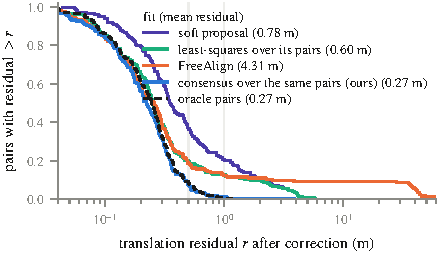
\includegraphics[width=\linewidth]{figures/residuals.pdf}
  \caption{\textbf{Blur, not error.} Fraction of dense \vxreal val pairs ($\sigma=\SI{2}{m}$, 194 pairs) whose translation residual after correction exceeds $r$. The proposal's correspondences are 95\% precise and 98\% complete, yet a least-squares fit over them leaves 13\% of pairs more than \SI{1}{m} off: a few wrong pairs carry full weight. A consensus fit over the \emph{same} pairs is the oracle-correspondence fit (\SI{0.27}{m} mean, 1\% over \SI{1}{m}); \freealign's \SI{0.26}{m} median hides a 12\% tail of wrong answers.}
  \label{fig:residuals}
\end{figure}

\subsection{Communication delay}
\label{sec:delay}
\begin{table}[t]
  \centering\small
  \caption{\textbf{Test under communication delay}, sweep means over $\sigma\in\{0,0.4,1,2\}$, 3 paired seeds; propose+verify+agree is the full method before the consensus floor. Last column: the full method.}
  \label{tab:delay}
  \resizebox{\linewidth}{!}{\begin{tabular}{llcccc}
    \toprule
    delay & metric & oracle & propose+verify+agree & \freealign & \paper \\
    \midrule
    \multicolumn{6}{l}{\textit{\vxreal}} \\
    \multirow{3}{*}{\SI{100}{ms}} & \ap{0.7} & .3421 & .2865 & .2842 & \textbf{.2968} \\
     & \ap{0.5} & .5588 & .4562 & .4428 & \textbf{.4728} \\
     & \ap{0.3} & .6075 & .5349 & .5124 & \textbf{.5509} \\
    \addlinespace
    \multirow{3}{*}{\SI{200}{ms}} & \ap{0.7} & .3189 & .2639 & .2574 & \textbf{.2755} \\
     & \ap{0.5} & .4815 & .4002 & .3846 & \textbf{.4182} \\
     & \ap{0.3} & .5673 & .4818 & .4540 & \textbf{.4982} \\
    \addlinespace
    \multirow{3}{*}{\SI{400}{ms}} & \ap{0.7} & .3136 & .2581 & .2529 & \textbf{.2711} \\
     & \ap{0.5} & .4463 & .3713 & .3604 & \textbf{.3891} \\
     & \ap{0.3} & .4880 & .4277 & .4040 & \textbf{.4433} \\
    \midrule
    \multicolumn{6}{l}{\textit{\opvv}} \\
    \multirow{3}{*}{\SI{100}{ms}} & \ap{0.7} & .3507 & .6383 & .6352 & \textbf{.6425} \\
     & \ap{0.5} & .8546 & .8624 & .8451 & \textbf{.8660} \\
     & \ap{0.3} & .9533 & .9280 & .9037 & \textbf{.9308} \\
    \addlinespace
    \multirow{3}{*}{\SI{200}{ms}} & \ap{0.7} & .2243 & .4976 & .4972 & \textbf{.5064} \\
     & \ap{0.5} & .4072 & .7191 & .7061 & \textbf{.7295} \\
     & \ap{0.3} & .7915 & .8539 & .8235 & \textbf{.8599} \\
    \addlinespace
    \multirow{3}{*}{\SI{400}{ms}} & \ap{0.7} & .2607 & .3873 & .3823 & \textbf{.4020} \\
     & \ap{0.5} & .3427 & .5644 & .5605 & \textbf{.5880} \\
     & \ap{0.3} & .4475 & .6935 & .6629 & \textbf{.7152} \\
    \bottomrule
  \end{tabular}}
\end{table}

Delay is not more localization error: static objects arrive correctly placed and moving ones displaced by their velocity times the delay, so no rigid correction repairs it and a solver must not be dragged off by the moving minority. Table~\ref{tab:delay} shows the ordering of Table~\ref{tab:thresholds} holds under delay on both datasets, at every $\sigma$ and every threshold. On \vxreal the full method leads \freealign by $+0.013$ / $+0.030$ / $+0.039$ \ap{0.7} / \ap{0.5} / \ap{0.3} at \SI{100}{ms} $+0.018$ / $+0.034$ / $+0.044$ at \SI{200}{ms} and $+0.018$ / $+0.029$ / $+0.039$ at \SI{400}{ms} (paired SE $\le 0.0006$): the lead grows from 100 to \SI{200}{ms} and holds at \SI{400}{ms}. On \opvv it leads by $+0.007$ / $+0.021$ / $+0.027$, $+0.009$ / $+0.024$ / $+0.036$ and $+0.020$ / $+0.028$ / $+0.052$ at 100 / 200 / \SI{400}{ms} (SE $\le 0.0006$), at every $\sigma$, and there the lead grows at every step. Huber IRLS down-weights the moving objects; \freealign's relative-distance graph has no equivalent, since one moving object changes its distance to every other node. The verify and agree stages are what make this hold: the per-pair rule of the deployed pipeline, which has neither, was \emph{behind} \freealign at \ap{0.7} under delay on \opvv ($-0.011$ / $-0.032$ / $-0.041$ on the sweep means against the same \freealign), since a fit that follows the moving majority most tightly scores best against a ground truth that does not move with it, and \freealign's fit is tighter than a soft proposal; the consensus fit over verified pairs is tighter still.

\subsection{\opvv: against intermediate fusion and \freealign}
\label{sec:opv2v}
\begin{table*}[t]
  \centering\small
  \caption{\textbf{\opvv test, \ap{0.7} against localization noise}, 2,170 frames, all methods under one detector range, one evaluator and paired noise draws. Intermediate-fusion methods from OpenCOOD checkpoints. Bytes per agent-frame: for intermediate fusion the float32 feature tensor each agent transmits at the fusion site, measured over 100 frames ($^\dagger$Where2comm: \SI{7.3}{MB} after its communication mask, 21\% rate); for the box-only aligners the overhead beyond the shared box payload of \SI{439}{B}, which is zero for both. \paper is the same rule as on \vxreal, selected jointly on both validation sets; 5 paired noise seeds for the box-only aligners.}
  \label{tab:opv2v}
  \begin{tabular}{lr*{8}{c}}
    \toprule
    $\sigma$ (m / deg) & bytes & 0 & 0.2 & 0.4 & 0.6 & 0.8 & 1.0 & 1.5 & 2.0 \\
    \midrule
    uncorrected late fusion & 0 & .8964 & .5978 & .3158 & .2154 & .1844 & .1763 & .1799 & .1898 \\
    F-Cooper~\cite{chen2019fcooper} & \SI{36.0}{MB} & .8402 & .7117 & .4445 & .2858 & .2037 & .1788 & .1506 & .1469 \\
    Where2comm~\cite{hu2022where2comm} & \SI{34.6}{MB}$^\dagger$ & .7849 & .7117 & .5851 & .4695 & .4106 & .3894 & .3851 & .4106 \\
    AttFuse~\cite{xu2022opv2v} & \SI{9.0}{MB} & .8638 & .7758 & .5983 & .5002 & .4648 & .4533 & .4447 & .4481 \\
    CoBEVT~\cite{xu2022cobevt} & \SI{34.6}{MB} & .8773 & .7824 & .5377 & .3807 & .2983 & .2746 & .2538 & .2544 \\
    V2VAM~\cite{li2023v2vam} & \SI{9.0}{MB} & .8975 & .8006 & .5702 & .4109 & .3385 & .3181 & .3410 & .3741 \\
    CoAlign fusion~\cite{lu2023coalign} & \SI{9.0}{MB} & .8831 & .7889 & .6150 & .5324 & .5090 & .5028 & .5023 & .5057 \\
    V2X-ViT~\cite{xu2022v2xvit} & \SI{8.7}{MB} & .8174 & .7894 & .7319 & .6732 & .6250 & .6027 & .5675 & .5515 \\
    \midrule
    \freealign~\cite{lei2024freealign} (pose-error-selected) & 0 & .8461 & .8334 & .8164 & .8094 & .8069 & .8054 & .8048 & .8047 \\
    \freealign (AP-selected, \SI{1.5}{m}) & 0 & .8406 & .8344 & .8236 & .8196 & .8178 & .8175 & .8174 & .8172 \\
    \paper, propose only & 0 & .8674 & .8359 & .8234 & .8185 & .8144 & .8137 & .8109 & .7976 \\
    \textbf{\paper} & 0 & .8526 & \best{.8433} & \best{.8320} & \best{.8282} & \best{.8277} & \best{.8264} & \best{.8262} & \best{.8252} \\
    \bottomrule
  \end{tabular}
\end{table*}
Table~\ref{tab:opv2v} is the comparison the bandwidth argument rests on. Every intermediate-fusion method is above the box-only aligners under exact poses, as it should be with a fused feature map of 8.7 to \SI{36}{MB} per agent-frame against \SI{439}{B} of boxes, and every one collapses from $\sigma=\SI{0.4}{m}$; V2X-ViT degrades most gracefully and is still 0.19 below \paper at \SI{2}{m}. Against \freealign re-selected on its own validation AP (\SI{1.5}{m}; its pose-error selection at \SI{0.5}{m} is 0.004 lower), the full method leads by $+0.0089\pm0.0001$ \ap{0.7} and 0.022 at IoU 0.5 and 0.3 on the sweep means, at every $\sigma$ including the clean case. The two tie on the 80\% of frames sharing three or more objects (.862 against .865 at \SI{2}{m}); the lead is the sparse bucket (13\% of test frames), where \freealign's graph is degenerate: .471 against .352 at \SI{2}{m}. The proposal stage alone, with its per-pair rule, is within 0.001 of \freealign; the weighted exact refit is what makes the difference on this dataset, because \opvv's detections are precise enough that an unweighted hard fit loses to the confidence-weighted soft one (Sec.~\ref{sec:ablation}).

\subsection{Ablations and selection}
\label{sec:ablation}
\begin{table}[t]
  \centering\small
  \caption{\textbf{Selection on \vxreal validation} (3 seeds, sweep-mean \ap{0.7}; paired SE $\le 0.0003$). Every row is one decision made before test.}
  \label{tab:ablation}
  \resizebox{\linewidth}{!}{\begin{tabular}{lcc}
    \toprule
    arm & \ap{0.7} & vs \freealign \\
    \midrule
    \freealign (AP-selected) & .3702 & \\
    propose, Wald 0.2 & .3456 & $-$.0246 \\
    + verify, ICP least squares, gates 2/1/0.5 & .3688 & $-$.0014 \\
    + verify, RANSAC, gates 2/1/0.5 & .3712 & +.0010 \\
    + verify, RANSAC, gates 4/2/1/0.5 & .3725 & +.0023 \\
    + verify, RANSAC, gates 6/3/1.5/0.75/0.5 & .3730 & +.0028 \\
    \quad + candidate search \SI{8}{m} / \SI{12}{m} & .3730 & +.0028 \\
    + agreement \SI{1.0}{m} & .3756 & +.0054 \\
    + agreement \SI{0.5}{m}, floor 4 & .3787 & +.0085 \\
    + agreement \SI{1.0}{m}, floor 6 & .3774 & +.0072 \\
    + agreement \SI{1.0}{m}, floor 4 & .3803 & +.0096 \\
    \quad gated on the Wald decision & .3720 & +.0012 \\
    \textbf{+ weighted exact refit} & \best{.3804} & \best{+.0097} \\
    \quad gated, weighted & .3721 & +.0014 \\
    \midrule
    pose-regression head (no matching) & \multicolumn{2}{c}{collapses to predict-zero} \\
    message + 128-d LiDAR embedding (per-pair arm: .3568 vs .3436 boxes-only) & \multicolumn{2}{c}{+.013 val, $\pm$.001 test} \\
    message + DINOv2 appearance head, verify arm (Sec.~\ref{sec:appearance}) & .3553 & $-$.0135 vs .3688 \\
    \bottomrule
  \end{tabular}}
\end{table}
Table~\ref{tab:ablation} is the record of every choice. The last four rows were selected jointly with \opvv validation under a rule fixed in advance, the largest mean over the two datasets of the paired lead over \freealign: on \opvv the unweighted refit lost 0.012 to \freealign, because its unweighted hard fit is less precise than the confidence-weighted soft one where detections are clean, and the weighted refit recovers 0.010 of that at no cost on \vxreal; gating the agreement rule on the Wald decision helps \opvv by 0.001 and costs \vxreal 0.008, and is not used. Three more things stand out. The hard fit is what matters, not its gate: the three RANSAC schedules are within 0.002 of each other and an explicit search for a better pose basin adds nothing on top of the widest. A direct pose-regression head, the design of the method we started from, never leaves the conditional mean on this data (yaw MAE equal to predicting zero at every $\sigma$), which is why yaw is solved analytically. And the per-object embedding that the message originally carried is within noise of the box-only trunk on both datasets and both splits with no stable sign, at 18 times the bytes; it was removed.

\subsection{Appearance does not help, and why}
\label{sec:appearance}
\begin{table}[t]
  \centering\small
  \caption{\textbf{Cross-agent identity from appearance on \vxreal validation.} AUC of same-object against nearest-neighbour pairs; the bar for a cue to be worth transmitting was 0.80 in both buckets.}
  \label{tab:appearance}
  \resizebox{\linewidth}{!}{\begin{tabular}{lccc}
    \toprule
    cue & dense pairs & sparse pairs & in the matcher \\
    \midrule
    colour histogram & .63 & -- & -- \\
    frozen ImageNet ResNet-18 & .60 & -- & $-$.012 \ap{0.7} \\
    DINOv2-B, zero-shot & .68 & .65 & -- \\
    + contrastive head, GT identities & .85 & .54 & -- \\
    + hard negatives, track pooling & .90 & .885 & $-$.011 \ap{0.7} \\
    + trained on detections & .84 & -- & $-$.011 \ap{0.7} \\
    \bottomrule
  \end{tabular}}
\end{table}
A natural reading of Table~\ref{tab:buckets} is that the sparse bucket needs an appearance cue to disambiguate the one or two shared objects. We tested it to the end. A cross-agent contrastive head on frozen DINOv2 patch features, with the nearest partner-frame vehicles as hard negatives and per-agent track pooling, separates cross-agent identities at AUC 0.885 on sparse pairs, well over the bar we set. Fed into the matcher as a 128-d per-object embedding it moves the sweep mean by $-$0.011 \ap{0.7} (+0.006 in the clean case). The mechanism is in the numbers: stage-1 association is 99.4\% Top-1 correct from geometry alone at the \SI{0.5}{m} noise stage~1 validates at, and Table~\ref{tab:association} shows the verified correspondences at 0.94 precision at every $\sigma$ with the oracle's residual on dense pairs, so there is almost nothing for appearance to fix, and the embedding's cost is pose-displaced tokens that the pose-invariant box geometry does not pay. The remaining gap to the oracle is solver precision on dense pairs, which the verification stage addresses with no new bytes.
